\documentclass[14pt, a4paper]{article}
\usepackage{mathtext}
\usepackage[T2A]{fontenc}
\usepackage[utf8]{inputenc}
\usepackage[russian]{babel}
\usepackage{multirow}
\usepackage{slashbox}
\usepackage{makecell}
\usepackage{graphicx}
\usepackage{physics}
\usepackage{amstext}
\usepackage{caption}
\usepackage{subcaption}
\usepackage{cmap}
\usepackage{float}
\usepackage{indentfirst}

\usepackage[a4paper,
            		left=1in,
            		right=1in,
           		 top=1in,
            		bottom=1in,
            		footskip=.25in]{geometry}

\renewcommand{\thesection}{\arabic{section}.}
\renewcommand{\thesubsection}{\arabic{section}.\arabic{subsection}.}

\title{\textbf{Отчет о выполнении лабораторных работ 6.1/6.2 "Генераторы синусоидальных колебаний с кварцевой стабилизацией частоты"}}
\author{Калашников Михаил, Б03-202б}
\date{}

\begin{document}
\maketitle

\section{Резонансный усилитель}

\begin{enumerate}

\item Соберем схему резонансного усилителя. Проведем измерения потенциалов на всех электродах транзисторов.

\begin{table}[H]
\centering
\begin{tabular}{ll}
$\phi_1=0\ В$, & $\phi_8=0\ В$, \\
$\phi_2=0.9\ В$, & $\phi_7=-8\ В$, \\
$\phi_3=-1\ В$, & $\phi_6=0.01\ В$, \\
$\phi_4=-1\ В$, & $\phi_5=-0.71\ В$. \\
\end{tabular}
\end{table}

По измерениям определим токи эмиттеров и крутизну транзисторов.
\[I_e=\frac{\phi_e}{2r_e+R},\quad r_e=25\ Ом,\ R=300\ Ом\]
\[I_{e, 1}=2.9\ мА,\quad I_{e, 2}=2\ мА\]

\[S=\frac{I_c}{U_T}\approx\frac{I_e}{U_T}\]
\[S_1=114\ кОм^{-1},\quad S_2=81\ кОм^{-1}\]

\item Подадим входной сигнал от генератора колебаний. По наблюдениям переменного напряжения на выходе найдем резонансную частоту: $\nu_р=1.14\ МГц$.

\item На резонансной частоте снимем амплитудную характеристику усилителя. Построим график зависимости коэффициентов усиления от амплитуды входного сигнала.

\begin{figure}[H]
\centering
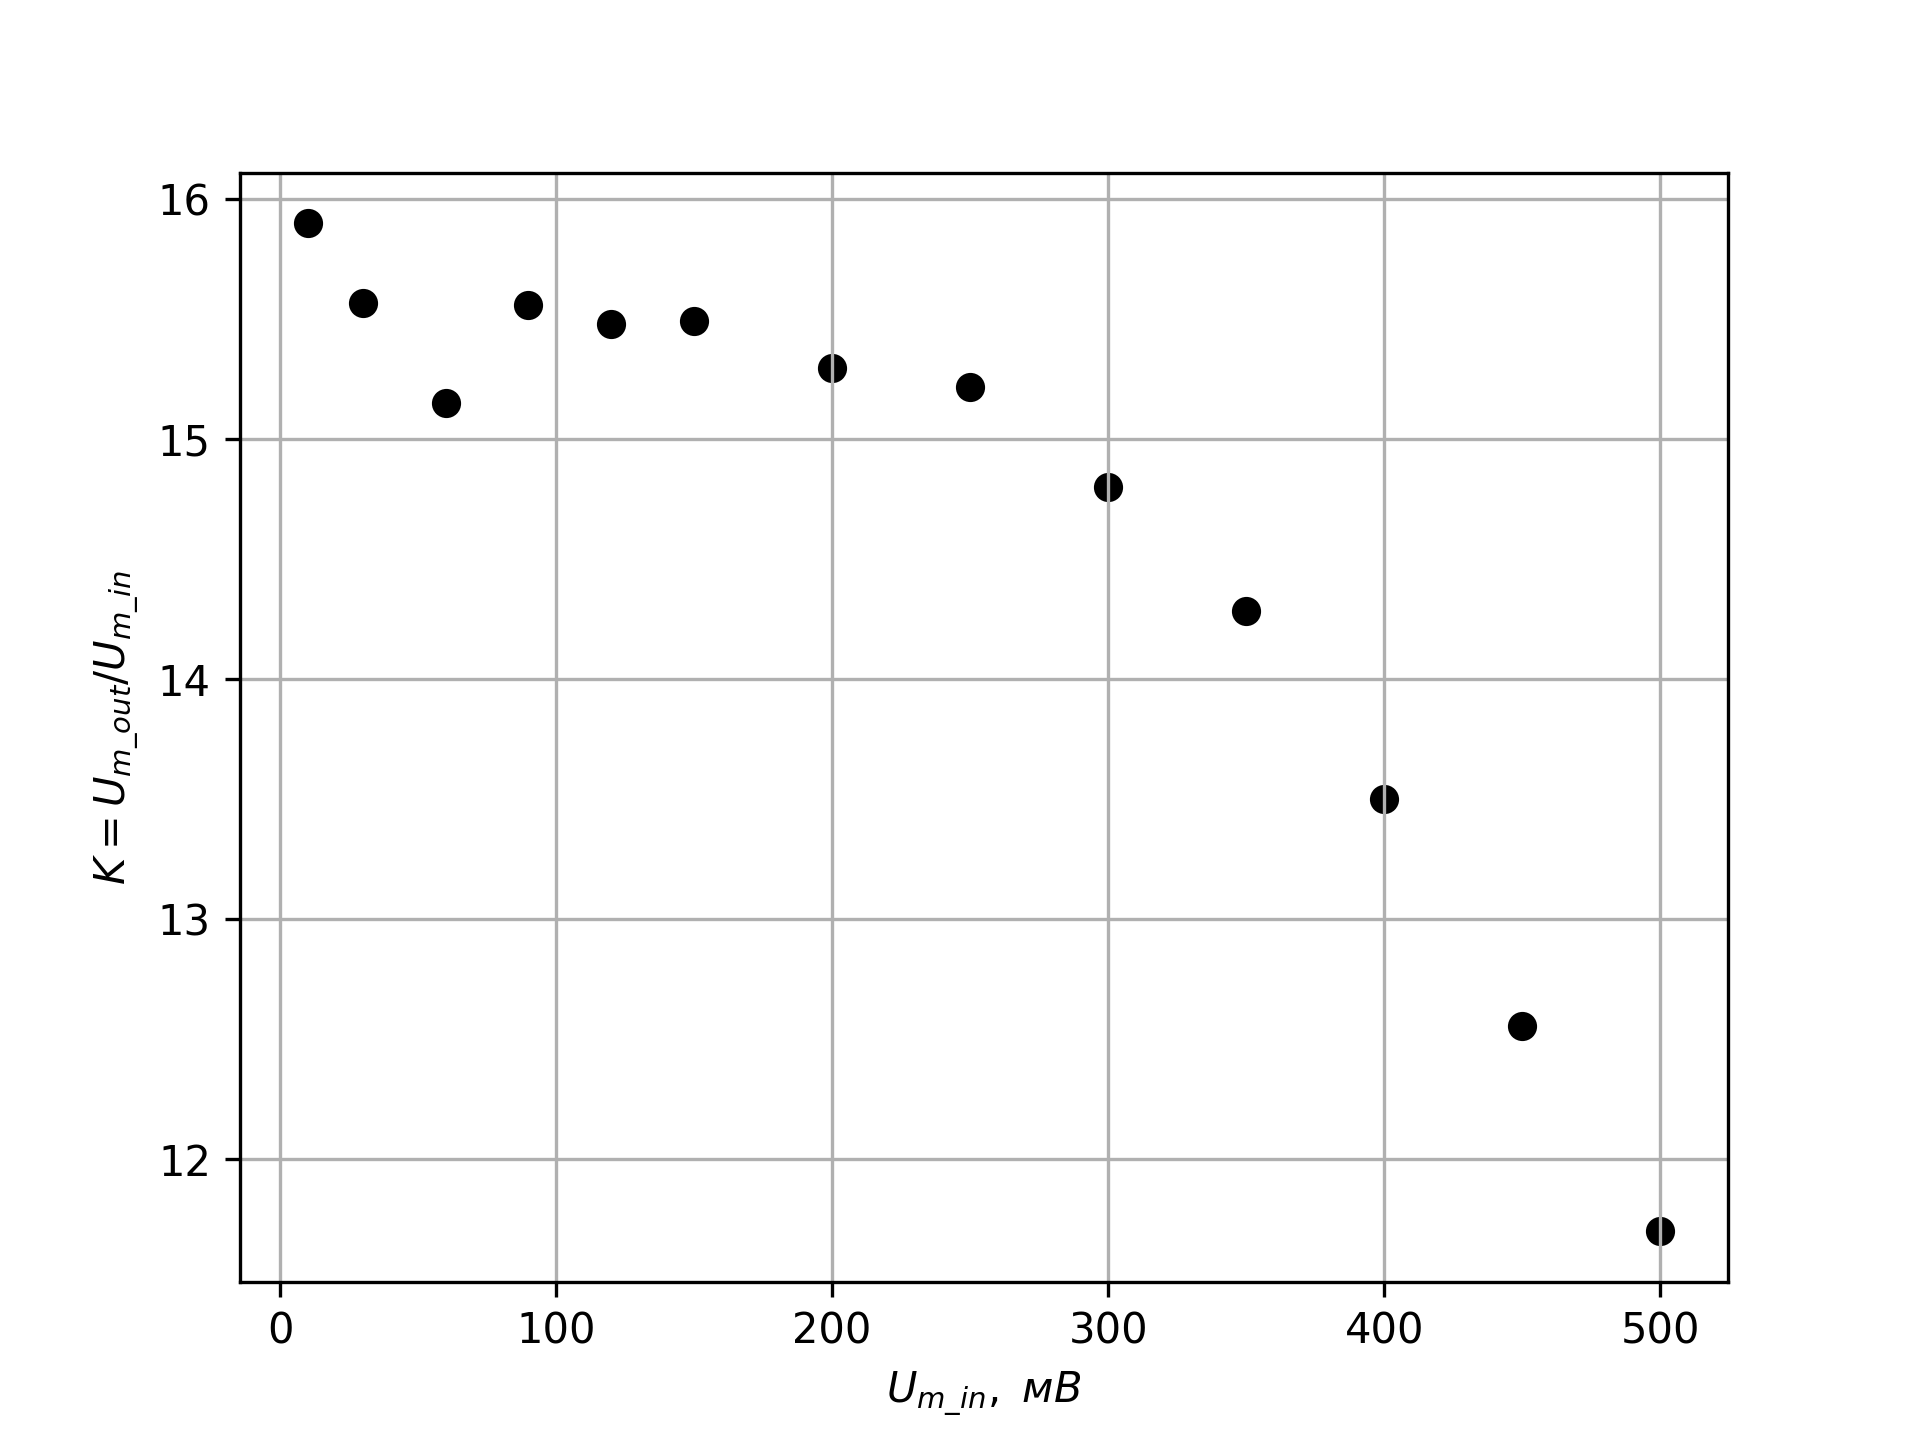
\includegraphics[scale=0.6]{../images/rt1-1}
\caption{Амплитудная харакетристика усилителя}
\end{figure}

\item Измерим резонансный коэффициент усиления для случая R=0, соединив эмиттеры транзисторов.

\item Снимем зависимость коэффициента усиления от частоты входного сигнала при амплитуде входного сигнала, соответствующей линейному амплитудной характеристики ($U_0=300 мВ$). Определим полосу пропускания на уровне 0.7 и добротность.

\begin{figure}[H]
\centering
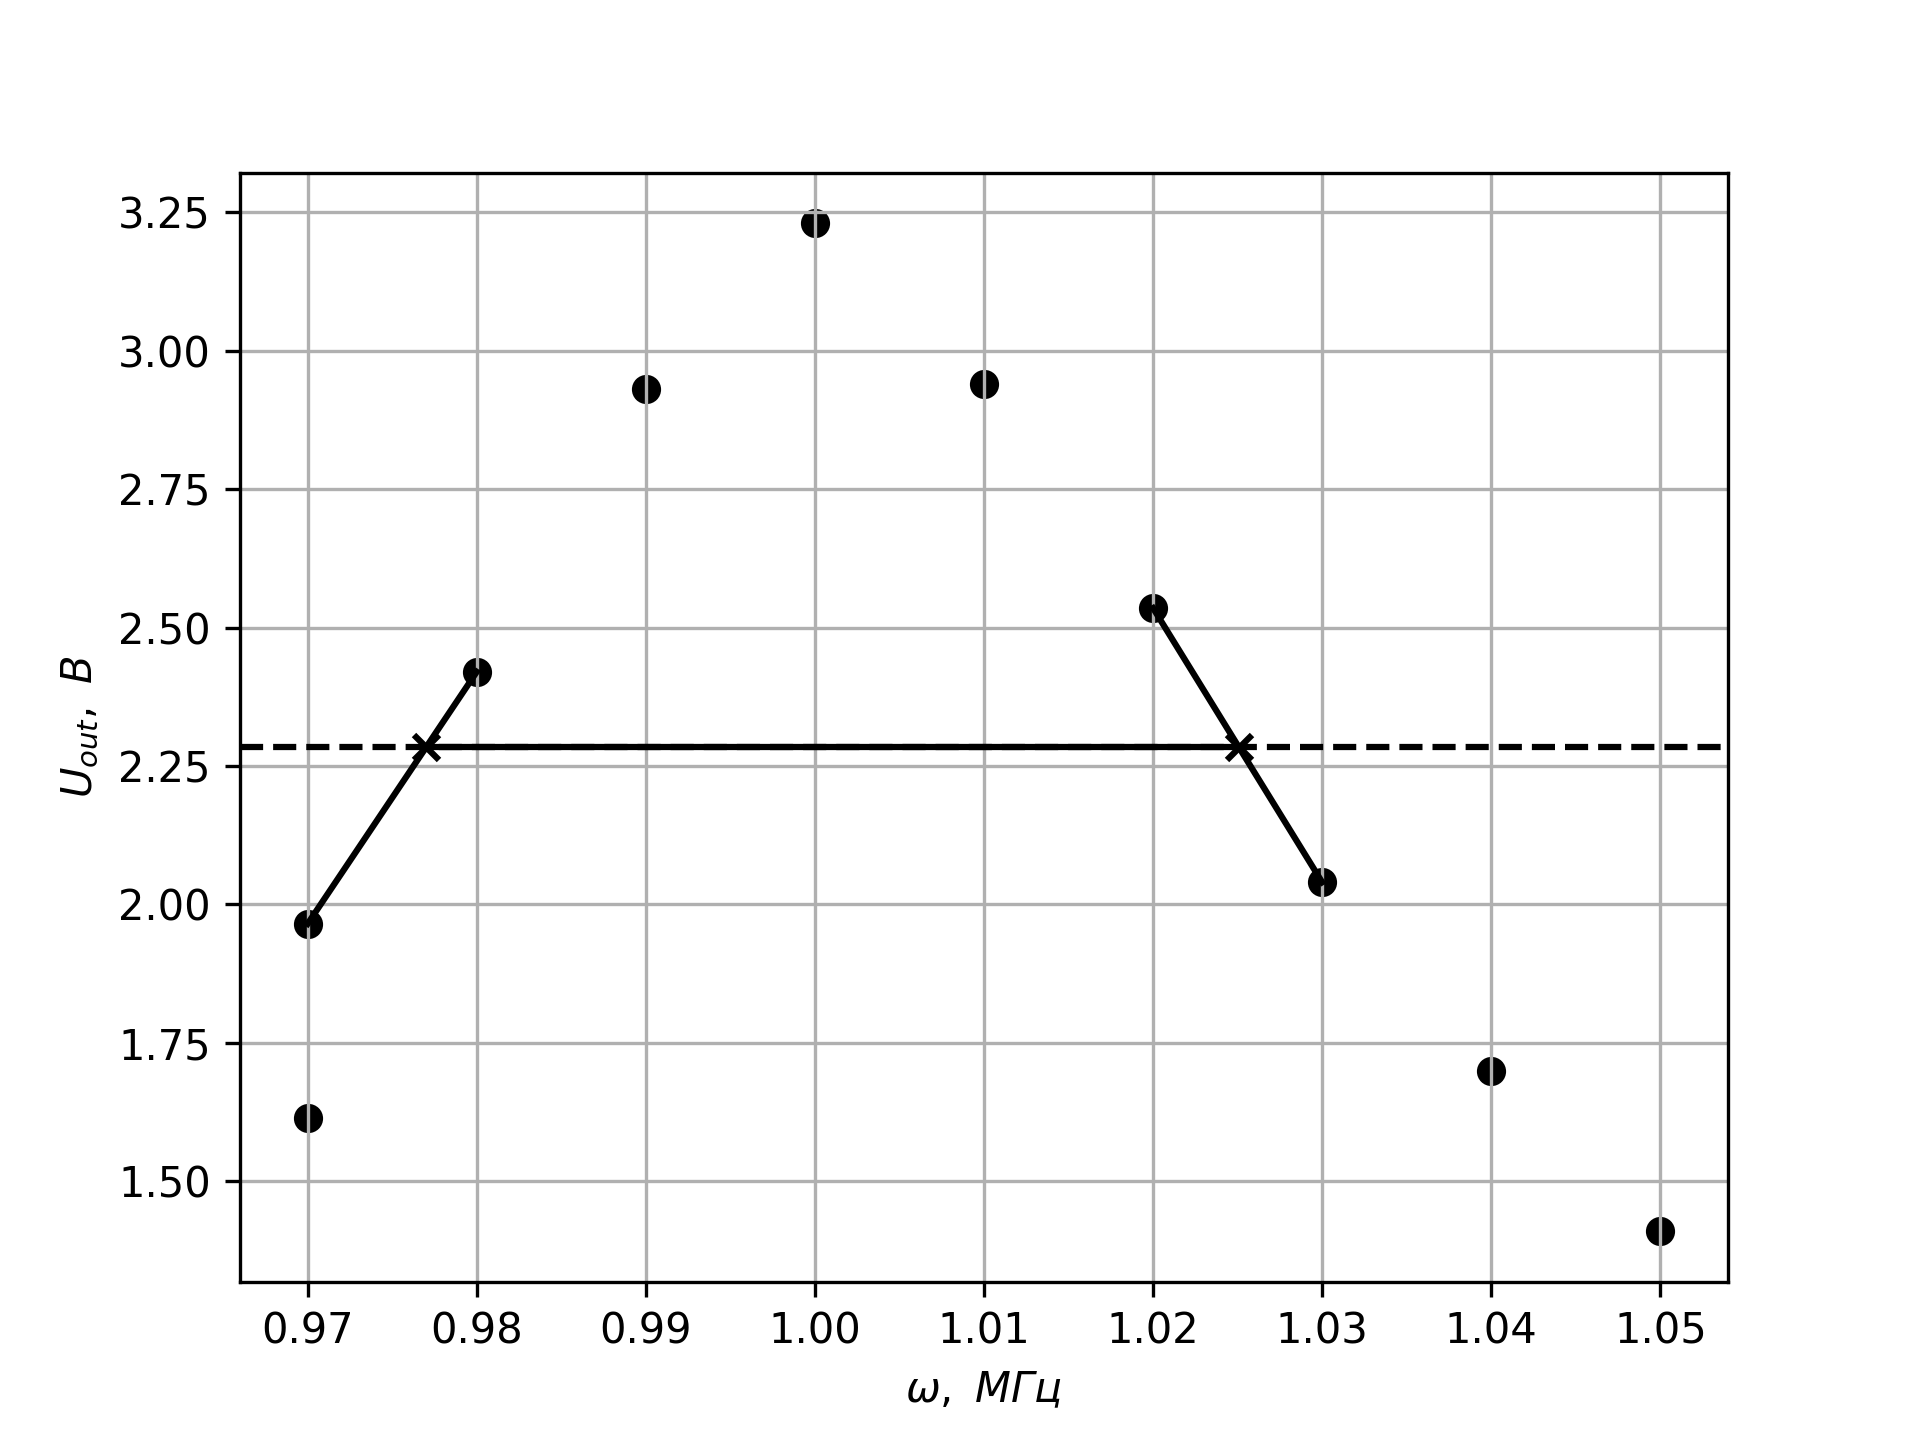
\includegraphics[scale=0.6]{../images/rt1-2}
\caption{Амплитудно-частотная харакетристика усилителя}
\end{figure}

Из графика получим, что $\Delta f_{0.7}=0.048\ МГц$, а $Q=f_{р}/\Delta f_{0.7}=20.8$.

\end{enumerate}

\section{Кварцевый генератор с использованием последовательного резонанса кварца}

\begin{enumerate}

\item Замкнем цепь обратной связи. Убедимся в наличии колебаний генератора без кварца. Подстройкой частоты добьемся чтобы частота колебаний была близка к 1 МГц. Измерим амплитуду выходного колебания: $U=1.6\ В$.

\item Заменим резистор между эмиттерами на кварцевый генератор. Измерим частоту колебаний: $\nu_р=1.004\ МГц$.

\item Измерим добротность кварцевого резонатора. Для этого проведем расстройку колебательного контура путем параллельного подсоединения дополнительного конденсатора емкости $\Delta C=15\ пФ$. После этого, $\Delta f_к=4\ Гц$, а $\Delta f=12\ кГц$.

Из соотношения $\Delta f_к/\Delta f=Q/Q_к$ определим добротность кварца $Q_к$:

\[Q_к=Q\frac{\Delta f}{\Delta f_к}=62400\]

\item Восстановим настройку контура в резонанс. Определим электричекие параметры кварцевого резонатора. Для этого последовательного с кварцем подключим конденсатор с емкостью $C_s=120\ пФ$ и измерим изменение частоты генерируемых колебаний $\Delta f_к=24\ Гц$. Рассчитаем параметры кварца по формулам:
\[C_к=2C_s\frac{\Delta f_к}{f_к}=0.0058\ пФ\quad, L_к=\frac{1}{4\pi^2 f_к^2 C_к}=4.4\ Гн\]
\[\rho_к=\frac{1}{2\pi f_к C_к}=27.6\ МОм\quad, r_к=\frac{\rho_к}{Q_к}=443\ Ом\]

\end{enumerate}

\end{document}